\subsection{Qué es una URL y una URL Maliciosa}

Una \textit{\gls{url}} (Uniform Resource Locator) es una dirección web que permite localizar y acceder a recursos en Internet. Las URLs son fundamentales para la navegación web, ya que especifican la localización de un recurso y el método para recuperarlo. Una URL típica puede descomponerse en varias partes, como se ilustra en la Figura~\ref{fig:partes_url}.

\begin{figure}[H]
    \centering
    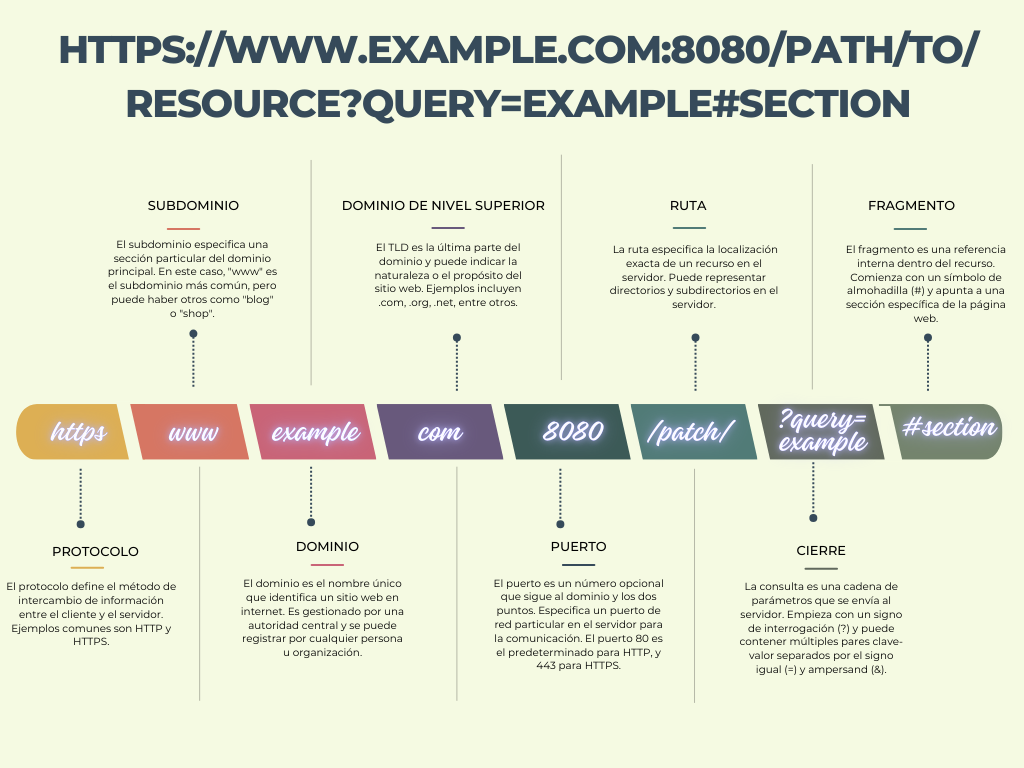
\includegraphics[width=0.8\textwidth]{urlPartes.png}
    \caption{Partes de una URL}
    \label{fig:partes_url}
\end{figure}

\begin{itemize}
    \item \textbf{Protocolo}: Define el método de intercambio de información entre el cliente y el servidor. Ejemplos comunes son HTTP y HTTPS.
    \item \textbf{Subdominio}: Especifica una sección particular del dominio principal.
    \item \textbf{Dominio}: Es el nombre único que identifica un sitio web en internet.
    \item \textbf{TLD (\gls{tld})}: Es el último segmento de un nombre de dominio.
    \item \textbf{Puerto}: Un número opcional que identifica una comunicación específica en el servidor.
    \item \textbf{Ruta}: Especifica la localización exacta de un recurso en el servidor.
    \item \textbf{Cierre}: Una cadena de parámetros que se envía al servidor.
    \item \textbf{Fragmento}: Una referencia interna dentro del recurso.
\end{itemize}

Una \textit{URL maliciosa} es una dirección web diseñada con la intención de engañar o perjudicar a los usuarios. Estas URLs son utilizadas por ciberdelincuentes para llevar a cabo ataques como \textit{\gls{phishing}}, distribución de malware, o redirección a sitios web fraudulentos. Las URLs maliciosas pueden parecer legítimas, imitando sitios web conocidos, o pueden tener componentes sospechosos como:

\begin{itemize}
    \item \textbf{Subdominios inusuales}: Para parecer confiables, algunas URLs maliciosas utilizan subdominios que imitan los legítimos.
    \item \textbf{TLDs no comunes}: Utilizan TLDs poco frecuentes para evadir filtros de seguridad.
    \item \textbf{Rutas y parámetros complejos}: Pueden incluir rutas o parámetros que parecen legítimos pero que redirigen a contenido malicioso.
    \item \textbf{Caracteres codificados}: Utilizan caracteres especiales o codificaciones que ocultan la verdadera intención de la URL.
\end{itemize}

La detección de URLs maliciosas es un desafío constante debido a la rapidez con la que estas pueden ser modificadas y la diversidad de técnicas utilizadas por los atacantes para evitar la detección. Nuestro estudio se enfoca en desarrollar métodos avanzados para identificar y mitigar estas amenazas a través de técnicas de \textit{machine learning} y análisis de características detalladas de las URLs.

